\section{Experimental Setup}
\label{sec:experiments}

This section describes the compute environment, datasets, experimental design, and sampling procedure used to evaluate the proposed diffusion-based kernel trace generator. All experiments use a unified training and generation pipeline and differ only in controlled variables such as temporal context length and feature availability.

\subsection{Compute Environment and Datasets}

All experiments were executed on the Nibi high-performance computing cluster. Each training and sampling job was allocated a single NVIDIA H100 GPU with 80\,GB of device memory, along with 8 CPU cores and 32\,GB of host memory. Mixed-precision training with \texttt{bf16} and TF32 acceleration was enabled to maximize throughput and maintain numerical stability on H100-class hardware.

We use windowed NPZ datasets derived from real LTTng kernel traces, as described in Section~\ref{sec:windowing}. Each dataset consists of fixed-length sequences extracted from the \texttt{all-events} tracing configuration and split into training, validation, and test partitions. Unless otherwise stated, experiments are conducted on the \texttt{scimark2} benchmark, which exhibits a diverse mix of compute, scheduling, and memory behavior and is commonly used in systems performance analysis.

\subsection{Model and Training Configuration}
\label{sec:model-config}

All experiments use the same diffusion-model architecture in order to isolate the effects of data representation and temporal context. The denoising network is a Transformer encoder with $d_{\text{model}}=512$, 8 attention heads, and 8 layers. The diffusion process uses $T=1000$ timesteps with a linear noise schedule. Optimization is performed using AdamW with a cosine learning-rate schedule. Aside from the experimental variables described below, all architectural and optimization hyperparameters are held constant across runs.

Table~\ref{tab:hyperparams} summarizes the model and training hyperparameters shared by all experiments.

\begin{table}[t]
\centering
\caption{Model and training hyperparameters (shared across all experiments).}
\label{tab:hyperparams}
\begin{tabular}{ll}
\toprule
\textbf{Parameter} & \textbf{Value} \\
\midrule
Model type & Transformer-based diffusion model \\
Embedding dimension ($d_{\text{model}}$) & 512 \\
Number of Transformer layers & 8 \\
Number of attention heads & 8 \\
Diffusion steps ($T$) & 1000 \\
Noise schedule & Linear $\beta$-schedule \\
Optimizer & AdamW \\
Learning-rate schedule & Cosine decay \\
Precision & bf16 (with TF32 enabled) \\
\bottomrule
\end{tabular}
\end{table}

\subsection{Experimental Design}

We conduct two complementary experimental studies: a \emph{context-length study} to evaluate scalability with respect to temporal context, and a \emph{feature ablation study} to quantify the contribution of system-level metadata.

\paragraph{Context-Length Study.}
To assess the impact of temporal context on generative fidelity, we train separate models using the full feature set (\texttt{event}, \texttt{dt}, \texttt{cpu}, \texttt{tid}, \texttt{comm}, \texttt{ret}) at three fixed sequence lengths: short (256), medium (1024), and long (4096). Batch sizes are adjusted per configuration to fit GPU memory constraints while maintaining comparable token throughput.

Table~\ref{tab:context-configs} summarizes the context-length configurations used in this study.

\begin{table}[t]
\centering
\caption{Context-length configurations for the scalability study.}
\label{tab:context-configs}
\footnotesize
\setlength{\tabcolsep}{4pt}
\begin{tabular}{lrrr}
\toprule
Configuration & $L$ & Batch & Tokens/batch \\
\midrule
Short context  & 256  & 256 & 65{,}536 \\
Medium context & 1024 & 128 & 131{,}072 \\
Long context   & 4096 & 32  & 131{,}072 \\
\bottomrule
\end{tabular}
\end{table}




This design enables a controlled comparison of short- and long-range dependency modeling while keeping all other architectural and optimization factors constant.

\paragraph{Feature Ablation Study.}
To isolate the effect of feature availability, we conduct a feature ablation study at a fixed sequence length of $L=1024$. We select $L=1024$ as a representative mid-range context that balances temporal coverage and computational cost: it is substantially longer than short-context settings while avoiding the high memory and training-time overhead of long-context configurations. Since context length is evaluated independently in the context-length study, fixing $L=1024$ prevents confounding the impact of feature removal with changes in temporal context.

At this fixed context length, we train separate models using progressively richer feature sets derived from the windowed NPZ representation. Table~\ref{tab:ablation-configs} summarizes the three ablation configurations used in our experiments.

\begin{table}[t]
\centering
\caption{Feature ablation configurations (fixed sequence length $L=1024$).}
\label{tab:ablation-configs}
\begin{tabular}{lcccccc}
\toprule
\textbf{Configuration} & \texttt{event} & \texttt{dt} & \texttt{cpu} & \texttt{tid} & \texttt{comm} & \texttt{ret} \\
\midrule
Base          & \checkmark & \checkmark & -- & -- & -- & -- \\
System-aware  & \checkmark & \checkmark & \checkmark & \checkmark & -- & -- \\
Feature-rich  & \checkmark & \checkmark & \checkmark & \checkmark & \checkmark & \checkmark \\
\bottomrule
\end{tabular}
\end{table}

This ablation isolates the contribution of scheduling context (CPU and thread identifiers) and semantic process metadata (command names and return values) to kernel trace realism and system-level validity.


\subsection{Sampling and Generation Protocol}

For each trained model, we generate synthetic kernel traces using the reverse diffusion process. Sampling starts from Gaussian noise and iteratively denoises for $T=1000$ steps. For consistency, models are re-instantiated with the same architectural hyperparameters used during training, and the corresponding checkpoints are loaded. Discrete channels are decoded using argmax over predicted logits, while continuous time-delta values are generated directly from the model output.

Synthetic traces are generated for all context-length and feature-ablation configurations and stored in the same windowed NPZ format as the real traces. These generated traces are evaluated independently against real data to assess how training and sampling configurations affect downstream fidelity and system-level validity metrics.

\paragraph{Constraint reference for evaluation.}
In addition to distributional comparisons against real traces, we evaluate system validity using a universal constraint knowledge base learned from the complete set of real NPZ shards (train/validation/test across dataset variants). All reported validity scores and repair experiments use the same \texttt{constraints\_universal.json} file to ensure consistent and reproducible assessment across models and configurations.

\subsection{Training Dynamics}

Training progress is monitored using TensorBoard, tracking the total diffusion loss as well as its latent and reconstruction components. Figure~\ref{fig:training-curves} shows representative training curves with and without exponential smoothing, demonstrating stable optimization and consistent convergence across all loss components.

To further compare convergence behavior across context-length configurations, Figure~\ref{fig:relative-training} presents the same losses visualized using TensorBoard’s relative-time view. These plots confirm that models trained with longer context lengths converge more slowly, as expected, but exhibit similarly smooth and monotonic loss reduction, indicating that increased temporal context does not introduce optimization instability.


\begin{figure}[t]
  \centering
  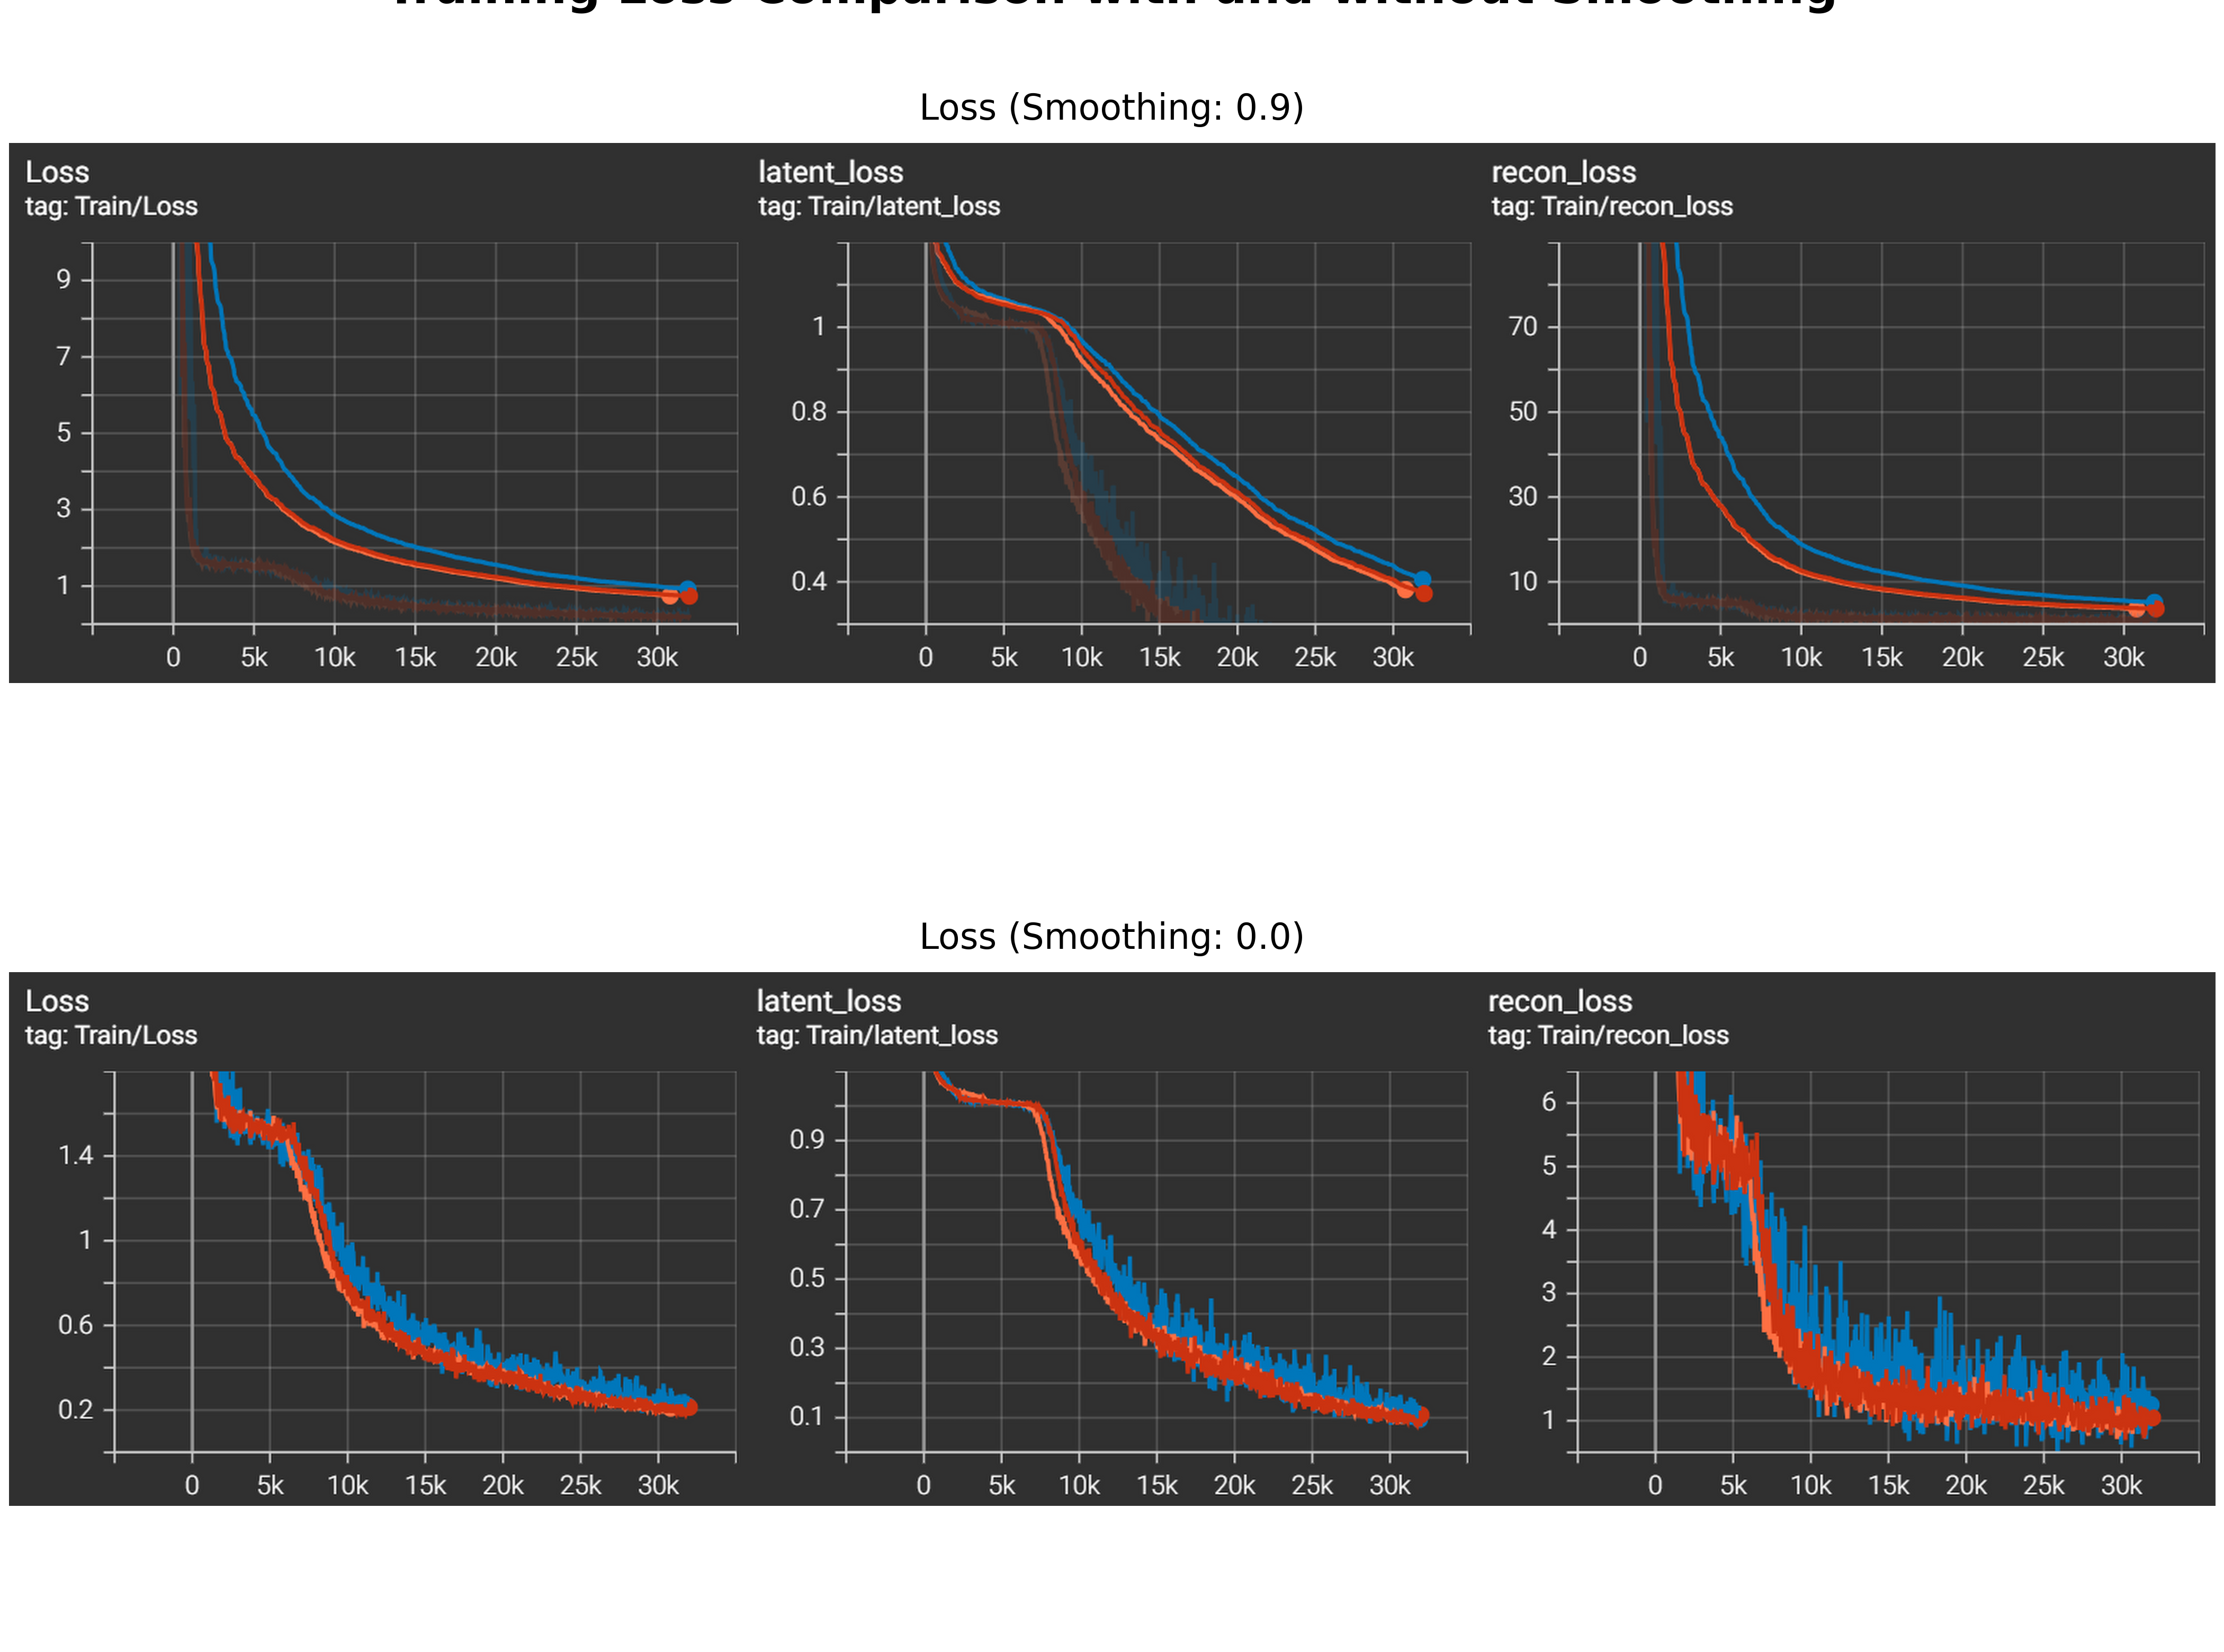
\includegraphics[width=\linewidth]{figures/loss_grid_comparison_compact.png}
  \caption{Training dynamics of the diffusion model.}
  \label{fig:training-curves}
\end{figure}

\begin{figure}[t]
  \centering
  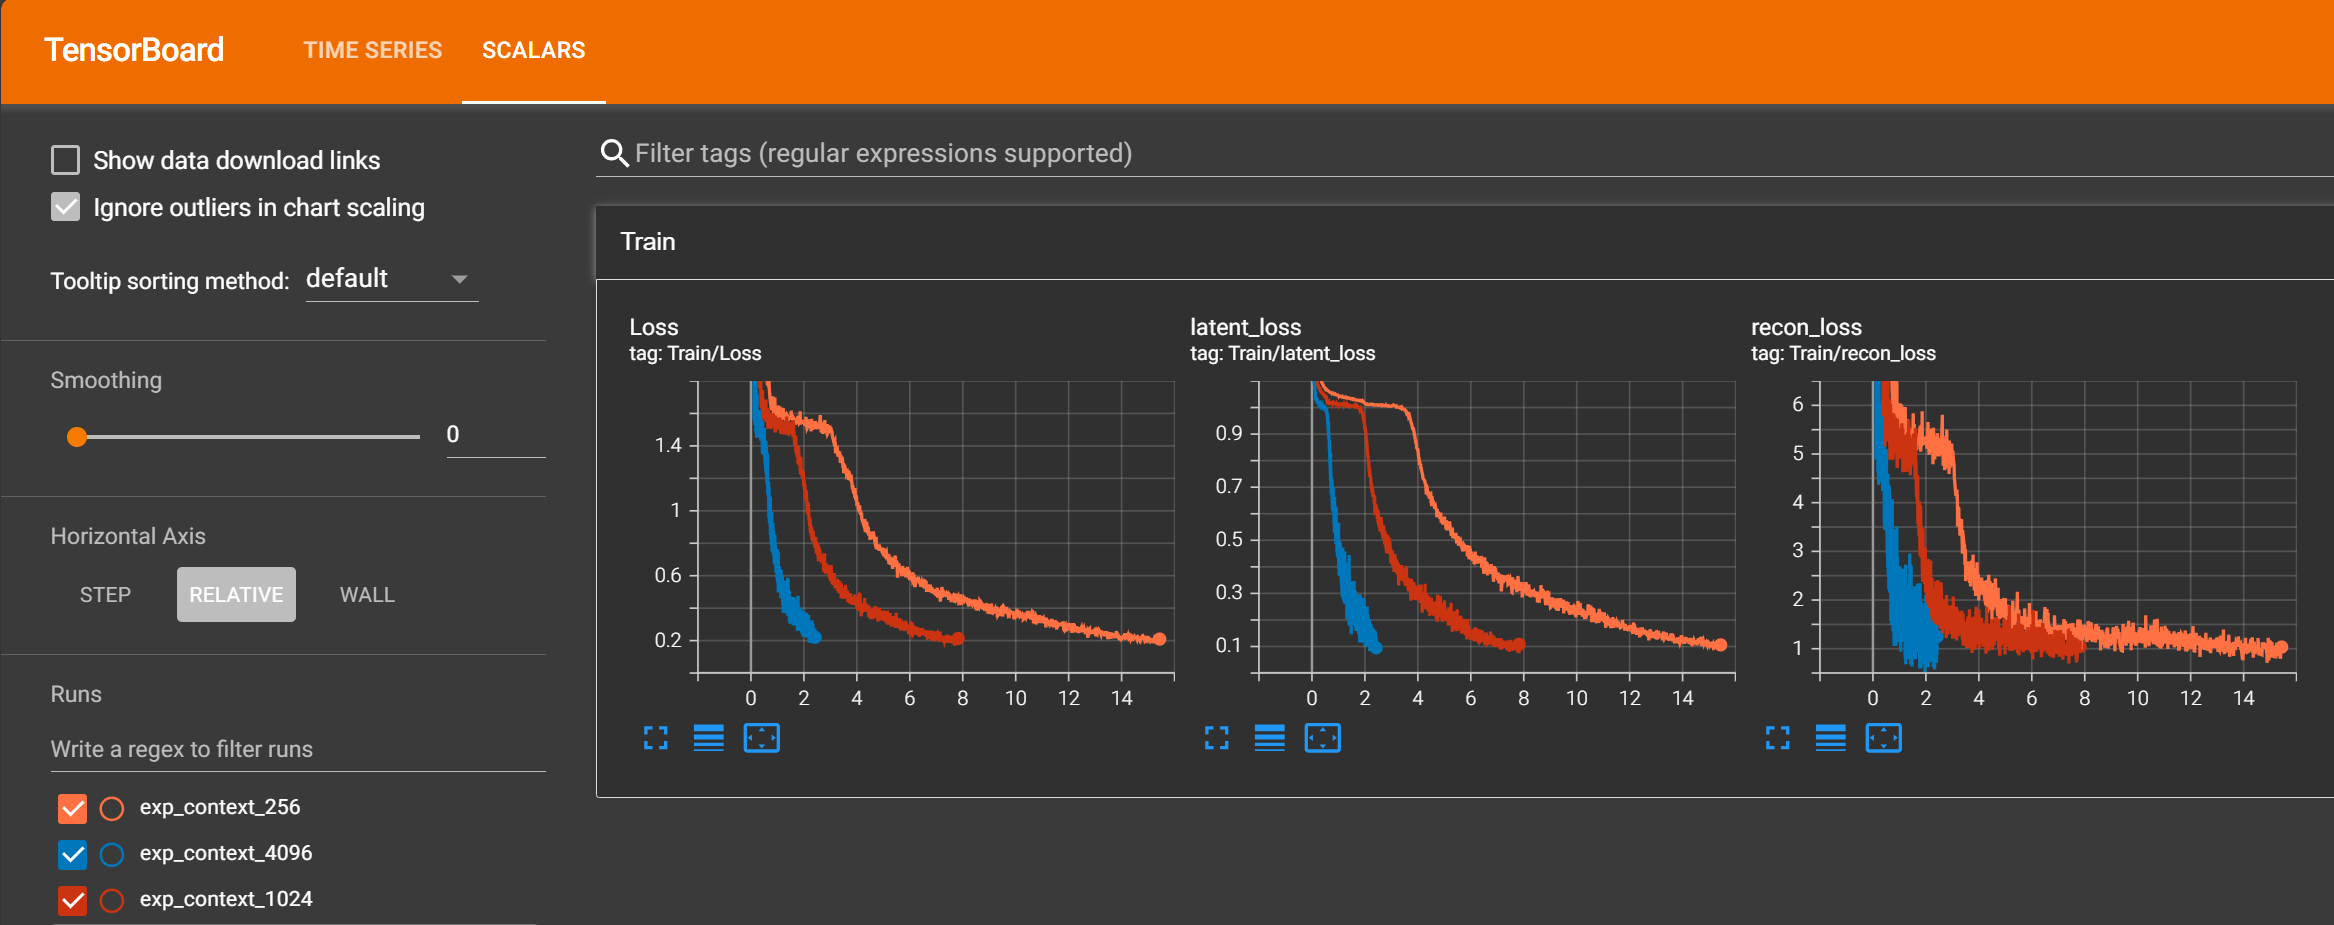
\includegraphics[width=\linewidth]{figures/relative-training-plot-2.png}
  \caption{Training loss visualized using TensorBoard’s relative-time view.}
  \label{fig:relative-training}
\end{figure}